\documentclass[10pt,twocolumn,letterpaper]{article}
\usepackage[T1]{fontenc}
\usepackage[review,applications]{wacv}
\usepackage{graphicx,booktabs,amsmath,amssymb,microtype,placeins}
\definecolor{wacvblue}{rgb}{0.13,0.34,0.54}
\usepackage[pagebackref,breaklinks,colorlinks,allcolors=wacvblue]{hyperref}
% Replace DRAFT with the assigned OpenReview paper identifier before submission.
% The WACV style option is distinct from choosing Vision4Neuro in OpenReview.
\def\wacvPaperID{DRAFT}
\def\confName{WACV}
\def\confYear{2027}
\title{Self-Supervised Skeleton Representations\\for Neurological Gait Analysis}


\author{Anonymous submission}
\begin{document}
\maketitle
\begin{abstract}
Learning useful descriptions of movement from limited video data could broaden access to quantitative behavioral analysis. We evaluate a compact Skeleton Joint Embedding Predictive Architecture (S-JEPA) on gait videos labeled Normal, multiple sclerosis, or Parkinson's disease. In each split, the encoder learns from 24 source videos, comprising 45--58 clips, by predicting hidden skeleton features without condition labels. A separate linear classifier uses its frozen features to predict collection labels for recordings excluded from training. Evaluation across five source-grouped folds covers 88 usable clips from 41 videos. S-JEPA achieves source-weighted macro-F1 of 0.457, compared with 0.325 for a Random Forest using handcrafted joint-angle features and 0.452 for mean pose. With equal weight per clip, S-JEPA also exceeds the Random Forest, scoring 0.397 versus 0.321. These results show that a compact predictive skeleton model trained on a small video collection can produce useful features for held-out label prediction. Mean pose remains a strong comparison, and further controls are needed to isolate the contribution of pretraining and temporal information. The study supports representation learning for markerless behavioral analysis, with clinical interpretation requiring recordings with verified diagnoses and participant identities.
\end{abstract}


\section{Introduction}
Walking provides an observable expression of motor function, making gait a useful subject for behavioral and clinical neuroscience. Multiple sclerosis (MS) can affect joint movement, stability and coordination in different combinations across individuals~\cite{filli2018,plotnik2020}. Video-based gait measurements have also been investigated in Parkinson's disease (PD)~\cite{shin2021}. These findings motivate the analysis of movement from ordinary recordings, where camera position, visibility and recording conditions accompany the movement of interest.

Markerless pose estimation converts video into trajectories of estimated body landmarks. Comparisons with reference measurements show that video-derived gait measures can be useful under specified recording and analysis conditions~\cite{stenum2021,stenum2024}. A common next step is to summarize these trajectories using quantities chosen in advance, such as joint angles and their ranges. Learning a representation directly from pose sequences offers another way to describe movement, without specifying every potentially useful relationship between landmarks.

Self-supervised methods create a training task from the observations themselves, allowing a model to learn features before condition labels are used. S-JEPA, introduced by Abdelfattah and Alahi, predicts features of hidden skeleton regions from visible context~\cite{sjepa}. Applying this framework to a small, heterogeneous gait-video collection tests whether the resulting features can be useful when few study-specific recordings are available.

We investigate whether a compact predictive skeleton model can produce useful representations from a small collection of gait videos. The model learns to predict hidden features of pose sequences without condition labels; a separate linear classifier then tests whether the frozen features contain information associated with the collection labels. Each encoder is trained on only 24 source recordings. Keeping all clips from a source together allows us to evaluate recordings that were excluded from both encoder and classifier fitting.

The main contribution is an empirical demonstration of useful trained features in this limited-data setting. S-JEPA exceeds a corrected Random Forest using handcrafted joint-angle summaries under both source-weighted and clip-weighted scoring. A mean-pose comparison helps assess how much can already be predicted from average pose without frame order, while a visibility-only comparison examines information available in the pose detector's outputs. These comparisons provide a case study of representation learning for markerless behavioral analysis and identify what remains to be tested before clinical interpretation.


\section{Related work}
\subsection{Video-based gait analysis}
Pose estimators such as BlazePose provide body landmarks from ordinary video~\cite{blazepose}.
Stenum et al. evaluated OpenPose-derived gait measures against reference measurements and extended this work across camera perspectives and clinical populations~\cite{stenum2021,stenum2024}. These studies establish the potential of video-based gait measurement while showing why the pose estimator, recording conditions, and intended measurement require validation. Their findings do not independently validate the BlazePose processing used in the present collection.


Shin et al.\ investigated quantitative gait analysis from single-camera videos of people with PD~\cite{shin2021}. Such studies connect defined video measurements to clinical or biomechanical references. The present collection instead supports a study of label prediction, because independently verified diagnoses and reference gait measurements are unavailable.

\subsection{Learning representations of movement}
SkeletonMAE learns representations by reconstructing masked skeleton information~\cite{skeletonmae}. MotionBERT learns motion representations by recovering 3D motion from partial or corrupted 2D observations~\cite{motionbert}. These methods motivate learning relationships among landmarks rather than relying exclusively on predefined summary features.

Kaur et al. used multi-view video and estimated 3D joints to classify gait from people with MS, PD, and matched older adults, including evaluations across participants and walking tasks~\cite{kaur2023}. GaitForeMer combined motion forecasting with activity classification during pretraining and then adapted its representations to PD gait-impairment severity~\cite{gaitforemer}. These studies place the present work within an existing line of learned neurological gait analysis. Our experiment examines a small collection of heterogeneous 2D web videos through a frozen-feature classifier; differences in labels, inputs, and evaluation designs prevent direct comparison of the reported scores.


\subsection{Predicting hidden features}
Wei et al. explored predicting features of masked image or video regions, including handcrafted image descriptors, as a way to learn visual representations without class labels~\cite{maskfeat}.


Joint-embedding predictive architectures learn by predicting feature vectors for hidden parts of an input from the visible context, as developed for images~\cite{ijepa}, video~\cite{vjepa} and skeletons~\cite{sjepa}. In S-JEPA, a second encoder supplies target features and is updated gradually from the context encoder. Prediction takes place in feature space, without reconstructing raw joint coordinates.

The original S-JEPA samples higher-motion tokens for hiding. Our compact adaptation uses 2D landmarks and detector visibility, with stochastic masks over anatomical regions. The experiment examines this trained representation in a small neurological gait-video collection; it does not compare the anatomical sampler with the original motion-based sampler.

\section{Dataset and preprocessing}
Figure~\ref{fig:pipeline} summarizes the procedure. We compiled 91 gait clips from 41 YouTube source videos found through searches for normal, MS and PD gait. Labels were assigned from video titles without independent clinical verification. Walking segments were selected manually: forward and return walks, or segments with different walking directions, could form separate clips. Footage with multiple people was cropped where needed to emphasize one person. Source-video identifiers retained in filenames group clips from the same recording.

The pretrained MediaPipe pose landmarker from the BlazePose family~\cite{blazepose} extracts 33 landmarks per sampled frame. Image coordinates are converted to pixels; horizontal and vertical coordinates and detector visibility are retained, while depth is discarded. Frame selection uses integer stride $\max(1,\operatorname{round}(f_{\rm src}/15))$, where $f_{\rm src}$ is the original frame rate. The target cadence is approximately 15 Hz, but the actual cadence depends on the original frame rate and integer sampling stride.

A clip is retained if at least 30\% of its sampled frames contain finite horizontal coordinates for every landmark and at least eight frames remain after cleaning. Empty ends are trimmed. Missing values are interpolated independently for each landmark and channel, boundary gaps receive the nearest observed value, and channels without observations are filled with zero. No maximum interpolation gap is imposed. Three clips are excluded, leaving 88 usable clips and all 41 sources (Table~\ref{tab:data}).

\begin{figure*}[t]
\centering
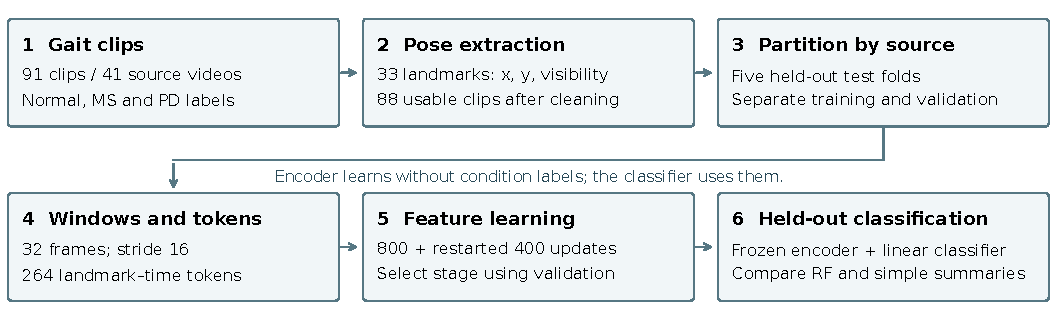
\includegraphics[width=\textwidth]{wacv-v1-revision-assets/pipeline.pdf}
\caption{From gait clips to held-out label prediction. All clips from one source recording remain in the same training, validation or test partition before windows are constructed. Each encoder is fitted on 24 source videos. The frozen-feature classifier uses collection labels, while the encoder's feature-learning objective does not. Validation selects between the two executed training stages. Baseline methods use the same source partitions.}
\label{fig:pipeline}
\end{figure*}

\begin{table}[t]
\centering\small
\setlength{\tabcolsep}{4pt}
\begin{tabular}{lrrrrr}
\toprule
Label & Raw & Usable & Sources & Padded & Windows\\
\midrule
Normal & 26 & 24 & 16 & 5 & 59\\
MS & 30 & 29 & 13 & 0 & 171\\
PD & 35 & 35 & 12 & 10 & 128\\
\midrule
Total & 91 & 88 & 41 & 15 & 358\\
\bottomrule
\end{tabular}
\caption{Dataset composition by collection label. Raw, usable and padded counts refer to clips. Sources are recordings, not verified participants. Windows contain 32 sampled frames and may overlap.}
\label{tab:data}
\end{table}

Let $h_t$ and $s_t$ denote the hip and shoulder midpoints in frame $t$. For S-JEPA and mean pose, landmark position $x_{tj}$ is normalized as
\begin{equation}
\widetilde{x}_{tj}=\frac{x_{tj}-h_t}{\max(\|s_t-h_t\|_2,10^{-3})}.
\label{eq:normalization}
\end{equation}
Visibility is unchanged. The RF branch calculates joint angles from cleaned pixel coordinates before this spatial normalization.

After source partitioning, each cleaned clip is divided into 32-frame windows with a stride of 16 frames; incomplete trailing windows are omitted. Window duration therefore varies across recordings. Clips shorter than 32 frames repeat their final frame to form one window, giving 15 padded clips in total. Padding does not add observed movement.

\section{Methodology}
\subsection{S-JEPA architecture}
An encoder converts the skeleton sequence into feature vectors. Four consecutive frames for one landmark form a token containing 12 values: horizontal position, vertical position and visibility in each frame. The 32-frame window therefore gives eight time blocks and $8\times33=264$ landmark--time tokens. A linear projection maps each token to 96 features, and learned landmark and time-position vectors identify its location in the sequence.

The context encoder combines information across visible tokens using three transformer layers with four attention heads. A two-layer transformer predictor, with separate positional vectors, estimates features at hidden positions. A target encoder with the same structure as the context encoder supplies the features to predict. It starts as a copy of the context encoder and processes the complete, untransformed training window. It receives no loss gradients; a moving average updates its weights from the context encoder. The skeleton model starts from fresh weights in each fold, while the upstream MediaPipe pose estimator is pretrained.

\subsection{Anatomical masking}
For each training window, the model predicts hidden features from the visible parts of the skeleton sequence. We sample masks over seven body regions: the head, mouth, left and right arms, trunk, and left and right legs. A selected region is hidden across one to six consecutive time blocks, and regions are added until approximately 60\% of the landmark--time tokens are hidden. Adding a whole final region can take the hidden fraction above 60\%; a check of 5,000 sampled masks gave an average of 63.2\%.

Regions containing any of 12 gait-relevant landmarks (Figure~\ref{fig:landmarks})---both shoulders, hips, knees, ankles, heels, and foot indices---receive a 1.5-fold multiplier in their selection weights, with an adjustment for overlapping region membership. The multiplier also affects the arm regions because they contain shoulders; it does not mean that every landmark in the selected set is hidden 1.5 times as often. All 33 landmarks can serve as visible context or hidden targets across successive masks. At least one token from the selected landmark set remains visible somewhere in each window.

This anatomical preference is motivated by the role of lower-limb movement and body coordination in gait~\cite{filli2018,plotnik2020}. The sampling checks verify how the masks are constructed; a separate comparison would be needed to determine whether the preference improves classification.


\begin{figure}[t]
\centering
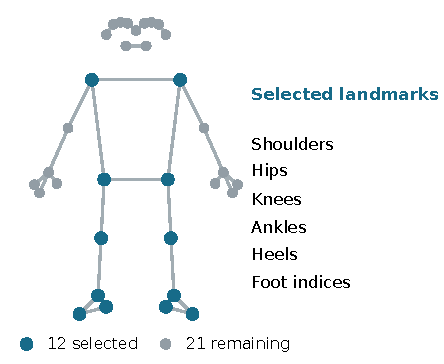
\includegraphics[width=0.93\columnwidth]{wacv-v1-revision-assets/landmarks.pdf}
\caption{BlazePose landmarks defining the anatomical sampling preference. Both shoulders, hips, knees, ankles, heels and foot indices belong to the selected set. Regions containing these landmarks receive increased selection weight, with an overlap adjustment; this does not prescribe a fixed hiding probability for individual landmarks. All 33 landmarks remain available. Schematic front view, with connections following BlazePose~\cite{blazepose}.}
\label{fig:landmarks}
\end{figure}

\subsection{Training strategy}
The encoder is trained on the Normal-, MS-, and PD-labeled videos in the training partition, without using their labels in the feature-learning objective. Each batch samples source videos with equal probability and then samples windows within those sources. This prevents recordings with more windows from dominating encoder training. Batches contain 32 windows.

The context encoder receives an augmented view with parts of the skeleton hidden, and the predictor estimates the target encoder's features at the hidden positions. Training compares distributions over feature dimensions using cross-entropy with centering and sharpening~\cite{dino}. These distributions describe learned features, rather than the three collection labels. Spatial augmentation uses rotation within $\pm15^\circ$, scaling from 0.9 to 1.1, translation within $\pm0.1$ normalized units, and horizontal reflection with probability 0.5. A single transformation is applied throughout each window. Reflection exchanges left and right landmark slots and visibility values, while the target window and target-mask positions remain unchanged. Its effect on side correspondence and useful gait asymmetry was not separately evaluated.

We train for 800 updates and evaluate a further 400-update continuation from the learned weights using the same training sources and objective. The continuation restarts the optimizer, running center, random-number generators and schedules. It therefore differs from uninterrupted training for 1,200 updates. For each stage, a linear classifier is fitted to the frozen features. The stage with higher source-weighted validation macro-F1 is selected, retaining the initial stage on a tie. Validation videos are excluded from encoder and classifier fitting, and test predictions are generated only after stage selection. The selected model is not refitted using the validation videos.


The supplementary material gives the loss equation, optimization settings and exact masking procedure.

\subsection{Frozen representation and classifier}
After training, the target encoder's weights are fixed. Each complete, unmasked window is passed through this encoder, and features at positions selected by one fixed sampled mask are averaged into a 96-dimensional vector. The mask selects outputs for averaging; it does not hide input landmarks during classification. Window vectors are then averaged to give one vector per clip. The same readout mask is used for all clips and folds, and sensitivity to that mask was not tested.

A scaler fitted on training clips standardizes the features, and logistic regression with $C=1$ and inverse-frequency class weights predicts the three collection labels. Each training clip contributes one observation. Thus, sources with more clips contribute more observations to classifier fitting, even though source videos are sampled equally during encoder training. Validation and test clips contribute to neither feature scaling nor classifier fitting.


\section{Experimental setup}
\subsection{Comparison methods}
The handcrafted Random Forest (RF) uses summaries of left and right hip, knee, and ankle angles, including mean angles, bilateral differences, and ranges of movement. The feature vector has 82 available fields, of which 15 angle statistics vary in this collection; the remaining fields are unpopulated or constant. Columns with no variation in the training partition are removed. A training-fitted scaler precedes an RF with 100 trees, maximum depth five, square-root feature subsampling, and balanced class weights. We use the corrected extractor with separate left- and right-ankle range features. An earlier implementation duplicated the right-ankle range, and its result is reported separately for transparency. This baseline summarizes lower-limb angles, whereas S-JEPA uses all 33 landmarks and visibility values, so the comparison evaluates these particular analysis pipelines.


Mean pose averages the normalized horizontal and vertical coordinates of all 33 landmarks across the full clip, giving 66 features without retaining frame order. The visibility baseline uses the mean and standard deviation of each landmark's visibility, also giving 66 features. Both use the same scaler and logistic-regression settings as the S-JEPA readout, fitted separately on the training clips. A majority-class baseline predicts the most frequent training-clip label. Mean pose uses coordinates alone, whereas S-JEPA also receives visibility.

\subsection{Source-grouped evaluation}
We divide the 41 source videos into five test folds, keeping the proportions of the three collection labels approximately balanced. Within the remaining sources, the first split of a stratified four-fold partition defines the training and validation sets. Each encoder and classifier is fitted using 24 source videos, comprising 45--58 clips depending on the fold (Table~\ref{tab:source_partitions}).

All clips and windows from a source remain in the same partition. Across the five test folds, every usable clip receives one prediction from a model that excluded its source from training and validation. This procedure separates identified source recordings; it cannot establish separation of participants who may appear in more than one source video.


An additional 8--9 sources per fold are used for validation, so fitting and stage selection together use 32--33 development sources. All methods share the same source partitions. The experiment uses training seed 42; it does not average multiple initializations. Keeping model selection separate from test evaluation follows the distinction emphasized by Varma and Simon~\cite{varma2006}.

\begin{table}[t]
\centering\small
\setlength{\tabcolsep}{5pt}
\begin{tabular}{lrrr}
\toprule
Fold & Training & Validation & Test\\
\midrule
0 & 24 / 51 & 8 / 19 & 9 / 18\\
1 & 24 / 58 & 9 / 17 & 8 / 13\\
2 & 24 / 54 & 9 / 17 & 8 / 17\\
3 & 24 / 53 & 9 / 21 & 8 / 14\\
4 & 24 / 45 & 9 / 17 & 8 / 26\\
\bottomrule
\end{tabular}
\caption{Sources / clips in each partition. Folds are numbered 0--4 throughout the paper and supplement.}
\label{tab:source_partitions}
\end{table}

\subsection{Evaluation measures}
We report macro-F1, which combines precision and recall separately for each collection label and then averages the three scores. Its range is zero to one, with larger values indicating better classification. The main score gives every source video equal total weight: a clip from a source containing $n$ usable clips receives weight $1/n$. Weighted prediction counts are combined across the five test folds before F1 is calculated. This prevents a recording with many clips from dominating the result.

We also report scores giving every clip equal weight and the number of correctly classified clips. These answer a different question because recordings contribute different numbers of clips. Fold results show how performance changes with the held-out recordings. Classes with undefined precision or F1 receive a value of zero. Supplementary material reports the resampling analysis and its scope.

\begin{figure*}[t]
\centering
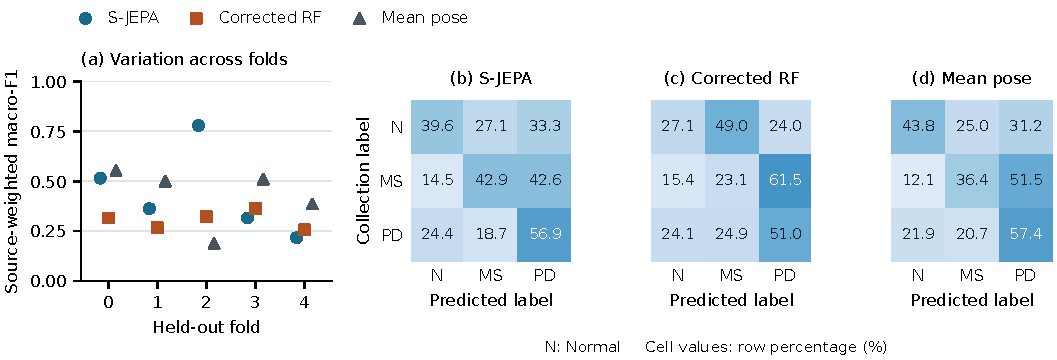
\includegraphics[width=\textwidth]{wacv-v1-revision-assets/results.pdf}
\caption{Held-out classification with equal total weight per source video. (a) Each fold uses the same test sources for all three methods; higher macro-F1 indicates better classification. The horizontal offsets separate the markers and do not represent additional folds. (b--d) Confusion matrices show the percentage assigned to each predicted label within each collection label. Every panel uses the same 0--100\% color scale; rows may not sum to 100 after rounding. RF uses the corrected bilateral ankle-range features.}
\label{fig:results_revised}
\end{figure*}

\section{Results}
\subsection{Classification using learned representations}
S-JEPA's frozen features support prediction of collection labels on recordings excluded from training. The pooled source-weighted macro-F1 is 0.457, compared with 0.325 for the corrected handcrafted RF (Table~\ref{tab:heldout_revised}), a difference of 0.131 on the F1 scale. With equal weight per clip, S-JEPA also exceeds RF, scoring 0.397 versus 0.321 and correctly classifying 36 of 88 clips compared with 30 for RF. Each encoder was trained on only 24 source videos.

Mean pose is a strong comparison, with source-weighted macro-F1 of 0.452. It exceeds S-JEPA with equal clip weighting (0.410 versus 0.397) and correctly classifies 37 clips. The small difference under source weighting therefore provides little basis for attributing S-JEPA's predictions specifically to temporal information. One MS-labeled source contributes 13 clips, illustrating why the two weighting schemes can produce different rankings.

\begin{table}[t]
\centering
\small
\setlength{\tabcolsep}{3pt}
\begin{tabular}{@{}p{0.43\columnwidth}rrr@{}}
\hline
Method & Source F1 & Clip F1 & Correct clips \\
\hline
S-JEPA + linear classifier & 0.457 & 0.397 & 36/88 \\
Joint angles + corrected RF & 0.325 & 0.321 & 30/88 \\
Mean pose + linear classifier & 0.452 & 0.410 & 37/88 \\
Visibility + linear classifier & 0.318 & 0.318 & 29/88 \\
Majority class & 0.259 & 0.202 & 23/88 \\
\hline
Earlier RF (duplicate) & 0.411 & 0.397 & 37/88 \\
\hline
\end{tabular}
\caption{Held-out classification of the collection labels. Macro-F1 combines predictions across all five test folds, weighting each source equally (Source F1) or each clip equally (Clip F1). Correct clips are unweighted counts. The final row records the earlier RF implementation with a duplicated ankle-range field; it is separate from the corrected main comparison.}
\label{tab:heldout_revised}
\end{table}

The earlier RF implementation scores 0.411 with source weighting. S-JEPA also exceeds that result, by 0.045, although the two clip-weighted scores round to 0.397 and the earlier RF is slightly higher before rounding. Correcting the ankle feature changes 12 RF predictions and lowers its score. The earlier and corrected executions use the same collection, partitions and seed, and produce identical S-JEPA predicted labels. They do not provide independent evidence across training seeds or datasets.

\subsection{Variation across recordings and labels}
S-JEPA exceeds corrected RF in three of five test folds, with fold macro-F1 ranging from 0.217 to 0.780 (Figure~\ref{fig:results_revised}). Mean pose exceeds S-JEPA in four folds. The higher pooled S-JEPA score reflects performance across all held-out predictions, including its strong result in fold 2, rather than a consistent advantage in every partition.

With equal source weighting, S-JEPA correctly identifies 39.6\% of Normal-, 42.9\% of MS-, and 56.9\% of PD-labeled examples, compared with 27.1\%, 23.1\%, and 51.0\% for corrected RF. PD predictions also include many examples from the other labels: their source-weighted precision is 38.6\%. In raw clip counts, S-JEPA correctly classifies 10 of 24 Normal clips, 8 of 29 MS clips and 18 of 35 PD clips; 13 MS clips are assigned to PD. The source-weighted percentages and raw counts use different weights. These errors limit clinical interpretation even though the features support useful prediction within this collection.

\subsection{Learning during training}
Training-batch feature-prediction loss decreases while the sampled target-encoder features retain variation across inputs. In the saved fold-0 training history, the first and last 50 updates of the initial stage have mean losses of 3.858 and 1.022, respectively. At the end of that stage, effective rank---a measure of how varied a batch of features is---is 12.13; the corresponding values across folds range from 10.90 to 12.13. Together with the held-out classifier results, these observations support the practical usefulness of the trained representation. They do not measure how much classification improved relative to an untrained encoder.

The continuation stage has a lower final training-batch loss in every fold, but improves source-weighted validation macro-F1 in only folds 3 and 4. The initial stage is retained in folds 0--2. Lower final training-batch loss therefore does not consistently coincide with better validation classification in this experiment; the validation step determines which stage is used for each test fold.




\section{Discussion}
\subsection{What the trained representation contributes}
The central finding is that a compact S-JEPA trained on a small collection of pose sequences produces features that support label prediction on held-out source recordings. A linear classifier using these features exceeds the evaluated handcrafted joint-angle RF under both source-weighted and clip-weighted scoring. This makes predictive skeleton learning a useful approach to investigate when large, clinically annotated movement datasets are unavailable.

The training history and downstream predictions provide complementary evidence. The training records show decreasing feature-prediction loss and nonconstant features on sampled training batches, while the frozen-feature classifier measures information associated with the collection labels. A matched untrained-encoder comparison would estimate the effect of pretraining on held-out label prediction under the same evaluation procedure. Mean pose's similar performance also leaves open the contribution of temporal order, as S-JEPA differs from that baseline in visibility inputs, feature dimension and the frames included in its window averages.

\subsection{Scope of the evidence}
The collection was assembled from publicly accessible gait videos, and its Normal, MS and PD labels were not independently clinically verified. Grouping by source video prevents clips from one identified recording from crossing partitions, but the same participant could appear in different recordings. Camera viewpoint, occlusion, pose-estimation errors and other recording characteristics may also contribute to prediction. The visibility-only classifier reaches source-weighted macro-F1 of 0.318. Whether this reflects a reproducible association with the collection labels, and whether movement or recording conditions contribute to that association, remains unresolved.

The RF comparison uses a specific set of lower-limb angle summaries, while S-JEPA uses all 33 landmarks and visibility. It therefore supports a comparison of these implemented pipelines, without establishing an advantage over every handcrafted gait analysis. The small number of training recordings also limits how confidently performance can be extended to new settings. Although the S-JEPA encoder is fitted on these recordings, its MediaPipe pose-estimation front end is pretrained; this is a small-data representation-learning experiment rather than a measurement of the full pipeline's data requirements.

Preprocessing further limits biomechanical interpretation. Centering on the hips and scaling by torso length remove absolute position and apparent body size, so the outputs are not calibrated measurements of walking speed or stride length. Missing detections are interpolated without a maximum gap length. Fifteen short clips are padded by repeating their final frame---five Normal and ten PD clips, with none from the MS collection---which can introduce label-associated temporal patterns. The minimum accepted clip length is eight sampled frames, so a clip need not contain a full gait cycle.

\subsection{Next comparisons}
The most informative next comparison would use the same architecture and readout with a randomly initialized encoder, followed by a supervised model trained on the same sources. Training and evaluating a matched model with shuffled frame order, while holding frames and visibility inputs fixed, would test whether temporal structure contributes to prediction. Comparing anatomical, unbiased regional and motion-based masking would assess the masking choice directly. Evaluation on recordings with verified diagnoses, participant identities and new acquisition settings would then test whether the learned features support reliable behavioral or clinical measurements.

\section{Conclusion}
S-JEPA produced useful features for gait-video label prediction after training on 24 source recordings per fold. Its frozen features, paired with a linear classifier, achieved source-weighted macro-F1 of 0.457, exceeding the corrected handcrafted joint-angle RF at 0.325 with performance close to the mean-pose comparison under both reported weighting schemes. This study establishes a practical small-data example of predictive representation learning for markerless behavioral analysis. Comparisons with untrained encoders and clinically verified recordings would clarify the contribution of pretraining and the relevance of these features to neurological movement assessment.


\FloatBarrier
\bibliographystyle{ieeenat_fullname}
\bibliography{wacv-v1-revision}
\end{document}
